% CVPR 2022 Paper Template
% based on the CVPR template provided by Ming-Ming Cheng (https://github.com/MCG-NKU/CVPR_Template)
% modified and extended by Stefan Roth (stefan.roth@NOSPAMtu-darmstadt.de)

\documentclass[10pt,twocolumn,letterpaper]{article}

%%%%%%%%% PAPER TYPE  - PLEASE UPDATE FOR FINAL VERSION
% \usepackage[review]{cvpr}      % To produce the REVIEW version
\usepackage{cvpr}              % To produce the CAMERA-READY version
%\usepackage[pagenumbers]{cvpr} % To force page numbers, e.g. for an arXiv version

% Include other packages here, before hyperref.
\usepackage{graphicx}
\usepackage{amsmath}
\usepackage{amssymb}
\usepackage{booktabs}
\usepackage{CJKutf8}
\usepackage{float}

% It is strongly recommended to use hyperref, especially for the review version.
% hyperref with option pagebackref eases the reviewers' job.
% Please disable hyperref *only* if you encounter grave issues, e.g. with the
% file validation for the camera-ready version.
%
% If you comment hyperref and then uncomment it, you should delete
% ReviewTempalte.aux before re-running LaTeX.
% (Or just hit 'q' on the first LaTeX run, let it finish, and you
%  should be clear).
\usepackage[pagebackref,breaklinks,colorlinks]{hyperref}

\usepackage{pifont}
\usepackage{xcolor}
\newcommand{\cmark}{\textcolor{green!80!black}{\ding{51}}}
\newcommand{\xmark}{\textcolor{red}{\ding{55}}}

% Support for easy cross-referencing
\usepackage[capitalize]{cleveref}
\crefname{section}{Sec.}{Secs.}
\Crefname{section}{Section}{Sections}
\Crefname{table}{Table}{Tables}
\crefname{table}{Tab.}{Tabs.}


%%%%%%%%% PAPER ID  - PLEASE UPDATE
\def\cvprPaperID{*****} % *** Enter the CVPR Paper ID here
\def\confName{CVPR}
\def\confYear{2022}


\begin{document}

%%%%%%%%% TITLE - PLEASE UPDATE
\title{Colorize B\&W Manga}

\author{Bing-Shu Wu,  Pin-Shao Chen\\
National Yang Ming Chiao Tung University \\
No. 1001, Daxue Rd. East Dist., Hsinchu City 300093, Taiwan\\
{\tt\small shu0924.cs09@nycu.edu.tw, cps@cs.nctu.edu.tw}
% For a paper whose authors are all at the same institution,
% omit the following lines up until the closing ``}''.
% Additional authors and addresses can be added with ``\and'',
% just like the second author.
% To save space, use either the email address or home page, not both
}
\maketitle

%%%%%%%%% ABSTRACT
\begin{abstract}
%   The ABSTRACT is to be in fully justified italicized text, at the top of the left-hand column, below the author and affiliation information.
%   Use the word ``Abstract'' as the title, in 12-point Times, boldface type, centered relative to the column, initially capitalized.
%   The abstract is to be in 10-point, single-spaced type.
%   Leave two blank lines after the Abstract, then begin the main text.
%   Look at previous CVPR abstracts to get a feel for style and length.
The purpose of this project is to colorize B\&W manga. We chose two ways, CNN and U-net, to be the models to train the agent. Refer to these two websites and this paper~\cite{CNN,U-net,Unet} to implement the CNN version and the U-net version. Finally, we improve the U-net version by putting the classifier in, which is referred by the website ~\cite{CNN}.
\end{abstract}

%%%%%%%%% BODY TEXT

\section{Introduction}
Coloring gray-scale images can have a big impact in many domains, for instance, understand historical images from a new perspective. This project is trying to color B\&W manga. We love watching anime and manga and want to see B\&W manga which have not be animated yet to be colorized. Hence by this opportunity, we try to make a tool that can colorize manga so that the manga matches the color of the anime.

Currently we know of the following ways to be models for colorize gray-scale images: CNN, U-net, GAN, Mask R-CNN. Finally chose CNN as the baseline and U-net as the main approach to colorize manga. Since these two methods are rarely mentioned in the course, it takes some time to learn and understand. We refer to this website~\cite{CNN} to implement the CNN version. Then refer to this paper~\cite{U-net} and this website~\cite{Unet} to understand and implement the U-net version. Finally, we have five different models to color manga. Then we compare the resulting photos with the photos that have been colored by existing programs in the Internet to see which one is the closest to the anime.

\section{Related Work}
We used the information of this website~\cite{CNN}, from the alpha version to the beta version, and gradually made the author's Full version. His beta version is a Sequential Model composed of Convolution 2D, while the full version is based on the beta version and add the Inception-ResNet-v2 model as a Classifier in the middle layer. In the end, we only retain the concept of Classifier, and choose the VGG16 model that is more suitable for our dataset. For the part other than Classifier, we implement a simplified version of the standard U-net structure.

This website~\cite{U-net} explains the U-net in detail and provides the relevant code, we reduced the number of filters to avoid hardware requirements of standard U-net exceeding the limit of our GPU. After combining the above two references, we also changed many parameters, such as learning rate, optimizer, activation function, etc., to optimize the coloring results.

\section{Methodology}
In order for the machine to learn how to color manga, we have to give it some examples of coloring. Then we use anime as the training dataset to train the models.

First, collect the data of anime. We write a simple program to screenshot once every two seconds. Play the anime and run the program until we get $600$ photos. Then randomly select $240$ images from it as the training dataset and $16$ images as the testing dataset. Then there is the data processing part. We directly use $skimage$ to resize the image to $256 \times 256$ to let the training process becomes faster. This is also to make the adjusted image size closer to the input image size $224 \times 224$ required by the VGG16 Classifier as our tool. And we also convert the color space of the picture from $RGB$ to $Lab$, $L$ is the corresponding graysacle value, so all the model has to do now is to predict the value of channel $a$ and channel $b$ for a given set of $L$ channels of size $256 \times 256$.

For the Evaluation Matrix, since there is no right or wrong in color, It is difficult to design a function to absolutely define the accuracy of an algorithm. Although this part can be measured by GAN, it is beyond the scope of our implementation. Therefore, we use the built-in CategoricalAccuracy() of $keras$ as our Evaluation Matric. After testing, this function does almost correctly reflect the status of a model. The principle of CategoricalAccuracy() is as Figure 1.

\begin{figure}[H]
\centering
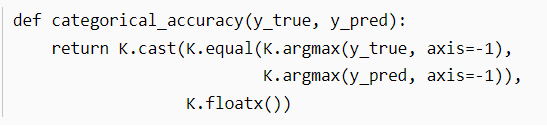
\includegraphics[width=0.4\textwidth]{fig1}
\caption{Categorical Accuracy}
\end{figure}

We can see that CategoricalAccuracy() will check for the innermost axis to check whether the maximum value of the prediction result (y\_pred) occurs at the same index as the  the real image (y\_true). We know that the matrix shape of the prediction result is $256 \times 256 \times 2$, where $256 \times 256$ is the image size, so the innermost axis is the value of $a$ and $b$ of $Lab$. Hence CategoricalAccuracy() can just measure whether the "relative color" is similar to the original image, rather than requiring the color to be absolutely consistent with the original image.

We use $keras$ and $tensorflow$ as model building tools to implement our baseline and main approach. These two methods have same difference from reference: our learning rate is very small. We found that the preset $0.001$ cannot be used as the learning rate, which will cause the results to not converge. The model will end the training process early and let every picture looks like yellowing photo. Therefore, we set the learning rate to $0.0001$, which makes the training results significantly improvement.

Baseline is a simple CNN, which is the Sequential Model we made with reference to~\cite{CNN}. The first half of the model adopts a design similar to the classifier which is to place Convolution 2D Layer and Max Pooling 2D Layer in. And the second half is to place the Convolution 2D Layer and Up Sampling 2D Layer in. The so-called Up Sampling 2D Layer is actually just copying the value of an element several times, as Figure 2. In this way, our baseline model is completed. The training process allows the machine to learn how to use the features learned in the first half and convert it into a color image output in the second half.

\begin{figure}[H]
\centering
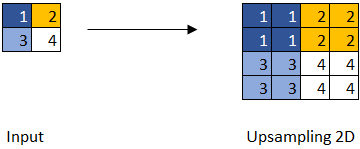
\includegraphics[width=0.4\textwidth]{fig2}
\caption{Up Sampling 2D Layer} 
\end{figure}

The Main approach is to make some changes with the baseline. We upgrade the simple CNN to U-Net, and connect the Layers of the first half and the second half. In addition, we directly added the ready-made VGG16 Classifier to the Layer in the middle. The concept here is like ordinary people learning to color. We must first know what an object is and what properties it has before we can draw a reasonable color. The model is no longer Sequential Model, it has two different inputs, one is our gray-scale image, and the other is the output of VGG16 Classifier, which is a $1 \times 1000$ one-dimensional array. 

The encoder (as figure 3) is similar to the first half of the baseline. In the decoder, compared with the second half of the baseline, we additionally use the concatenate layer to connect the decoder with the same-level encoder, and replace the Upsampling2D Layer with a learnable Transpose Convolution 2D Layer. The middle of the model is to combine the the output of the encoder with the output of the classifier. Since Maxpooling2D $((2, 2))$ appears $4$ times in the encoder, the output shape of the encoder will be $\frac{256}{2^4} \times \frac{256}{2^4} \times$ filter\_num, which is $16 \times 16 \times$ filter\_num. Hence Repeat Vector repeats the VGG16 output in $16 \times 16$ times, then reshapes it into a shape of $16 \times 16 \times 1000$. Finally, we uses the concatenate layer to combine the output of the encoder with the output of the  repeated and reshaped VGG16 Classifier, and then add two layers of Convolution 2D to complete the middle part.

\begin{figure}[H]
\centering
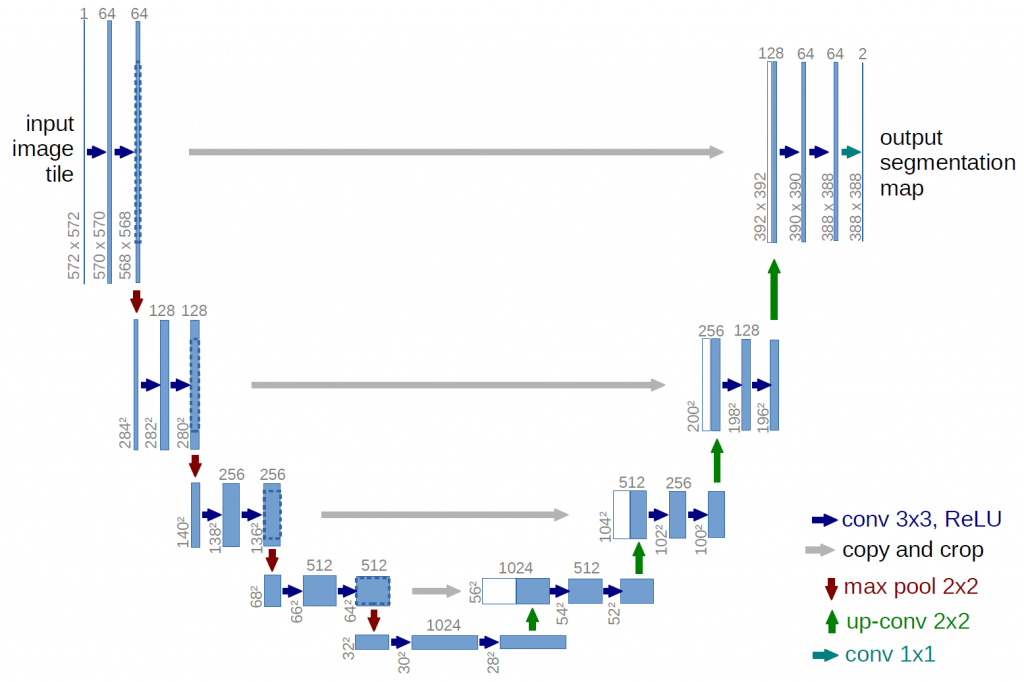
\includegraphics[width=0.4\textwidth]{fig3}
\caption{U-net (the left half is called the encoder, the right half is called the decoder, and the connection method is the gray arrow.)} 
\end{figure}

Finally, we replace all ReLU by LeakReLU (alpha=$0.2$) in the models to let activation function not to be too monotonous. This change makes the results better and less likely to fall into local optimal, but the hardware requirements will be higher.

\section{Experiments}

After training, agent can infer the testing dataset. We compare beta\_v2(baseline, epoch=200, batch size=16) and u-net LeakReLU (main approach, epoch=200, batch size=8) for the following examples. By the way, it has been tested that when the batch size is larger, it will have better results, but if batch size is too large, it will be limited by the hardware and cannot be trained. 

For Accuracy, as shown in Figure 4, main approach (b) have higher value of test data than baseline (a).

\begin{figure}[H]
  \centering
  \begin{subfigure}[b]{0.45\linewidth}
    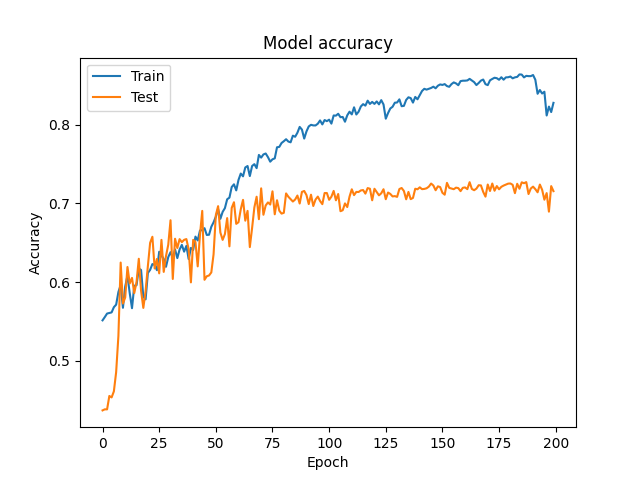
\includegraphics[width=\linewidth]{fig7}
     \caption{CNN beta\_v2}
  \end{subfigure}
  \begin{subfigure}[b]{0.45\linewidth}
    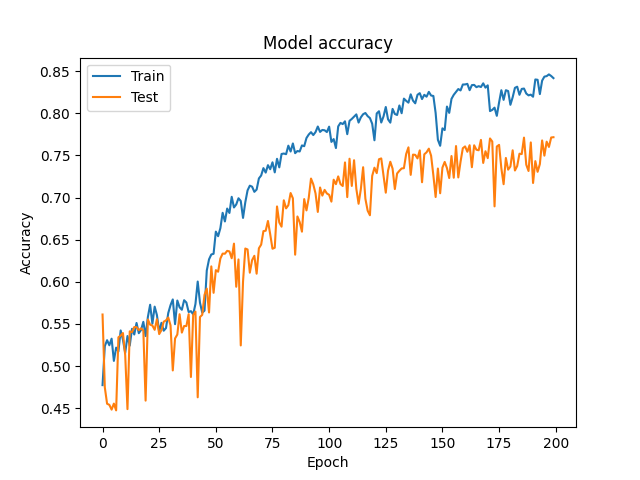
\includegraphics[width=\linewidth]{fig4}
    \caption{U-net LeakReLU}
  \end{subfigure}
  \caption{Accuracy}
\end{figure}

For their MSE Loss, as shown in Figure 5, obviously (b) converges better than (a). Then enlarge Figure 5, as shown in Figure 6, which help us to see the detail of (b). This can help us to compare the convergence of the baseline and the main approach.

\begin{figure}[H]
  \centering
  \begin{subfigure}[b]{0.45\linewidth}
    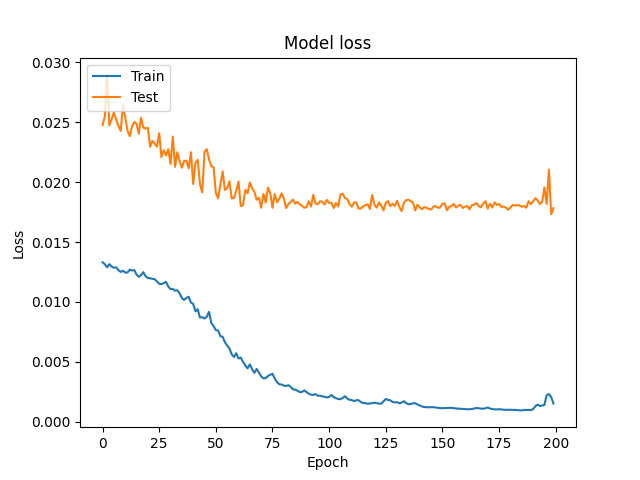
\includegraphics[width=\linewidth]{fig8}
     \caption{CNN beta\_v2}
  \end{subfigure}
  \begin{subfigure}[b]{0.45\linewidth}
    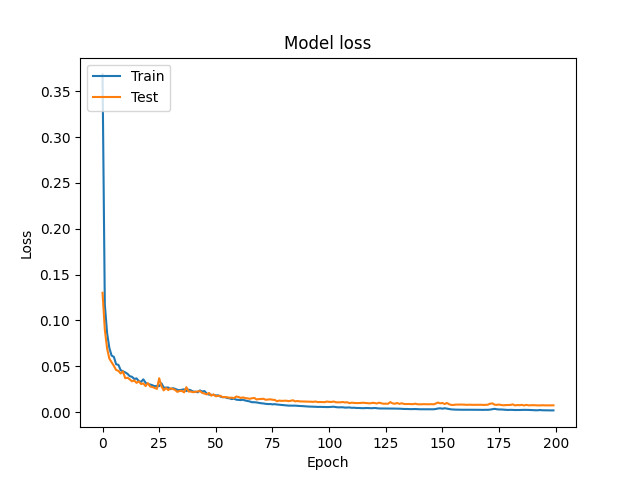
\includegraphics[width=\linewidth]{fig5}
    \caption{U-net LeakReLU}
  \end{subfigure}
  \caption{Loss (MSE)}
\end{figure}

\begin{figure}[H]
  \centering
  \begin{subfigure}[b]{0.45\linewidth}
    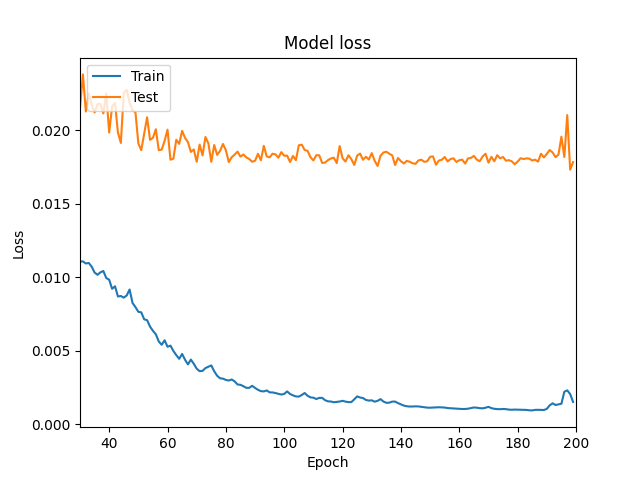
\includegraphics[width=\linewidth]{fig9}
     \caption{CNN beta\_v2}
  \end{subfigure}
  \begin{subfigure}[b]{0.45\linewidth}
    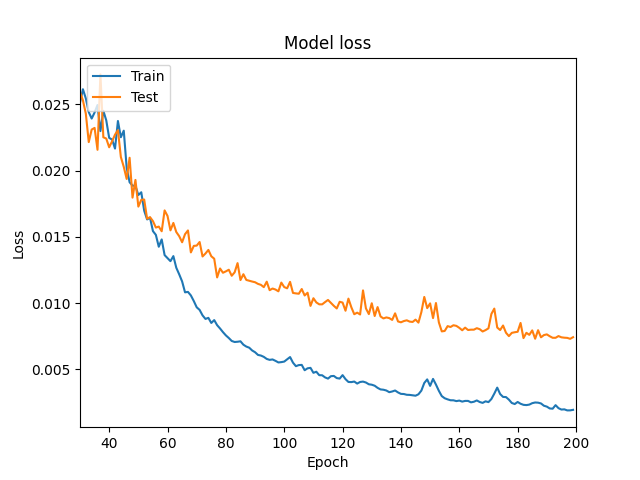
\includegraphics[width=\linewidth]{fig6}
    \caption{U-net LeakReLU}
  \end{subfigure}
  \caption{Loss after 30 epoch}
\end{figure}

There is still a lot of direction for research on Image Colorization, such as adding GAN to determine whether a prediction result is a reasonable coloring to replace the rough MSE loss, or using Mask R-CNN to see if the result will be better than U-net or not. 

In the end, we try to use above agent to color manga, However, the result is not very ideal. Instead, the effect of the app on the Internet is better, probably because the agent on the Internet has a higher degree of learning, and able to identify various objects and give relatively reasonable colors. But the problem remains that the colors may deviate from the anime's color scheme. Based on the fact that we don't have such good hardware for the agent to learn, we may reconsider whether there are other ways in the future.

%-------------------------------------------------------------------------

%%%%%%%%% REFERENCES
{\small
\bibliographystyle{ieee_fullname}
\bibliography{egbib}
}

\end{document}
